% 依固定扫描页重绘；两平面以平行四边形示意，交棱为 PQ，A 在平面 α 内，B 在平面 β 内，C 在 PQ 上。
% 面片与投影仅为拓扑示意，不按比例；不编码题面未给出的长度、角度、垂足或点 O 的定义。
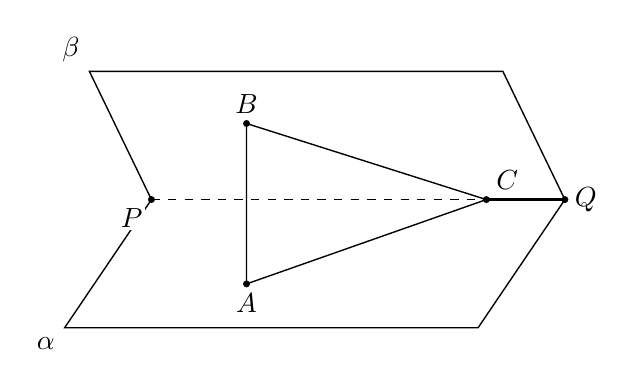
\begin{tikzpicture}[line width=.5pt,scale=1.05]
  \coordinate (P) at (0,0);
  \coordinate (Q) at (5,0);
  \coordinate (BtL) at (-.75,1.55);
  \coordinate (BtR) at (4.25,1.55);
  \coordinate (AlL) at (-1.05,-1.55);
  \coordinate (AlR) at (3.95,-1.55);
  \coordinate (A) at (1.15,-1.02);
  \coordinate (B) at (1.15,.92);
  \coordinate (C) at (4.05,0);
  % 两个平面以平行四边形作投影边界，共用棱 PQ。
  \draw (P)--(BtL)--(BtR)--(Q);
  \draw (P)--(AlL)--(AlR)--(Q);
  \draw[dashed] (P)--(C);
  \draw[thick] (C)--(Q);
  % 原图中的三角形 ABC 与交棱关系。
  \draw (A)--(B)--(C)--cycle;
  \fill (P) circle (1.2pt) (Q) circle (1.2pt) (A) circle (1.2pt)
    (B) circle (1.2pt) (C) circle (1.2pt);
  \node[fill=white,inner sep=1pt,below left=2pt] at (P) {$P$};
  \node[right] at (Q) {$Q$};
  \node[below] at (A) {$A$};
  \node[above] at (B) {$B$};
  \node[above right] at (C) {$C$};
  \node[above left] at (BtL) {$\beta$};
  \node[below left] at (AlL) {$\alpha$};
\end{tikzpicture}
